\section{Additional MCR Study Evidence and Open Decisions}\label{app:new-evidence}
This appendix identifies the new data files supplied for the MCR. The plots and tabulated results are outputs of the supplied study files and do not establish final payload calibration, a new launch epoch, or compliance with spacecraft requirements by themselves.

\subsection{Science grid and mission-tier studies}
The MMSC, MSC and EMSC grid-disposition outputs are based on different cell grids and modeled geographic domains. ``Primary Map'' is the disposition assigned in each output file, not a declaration of global requirement closure. The table summarizes the file contents directly.

\begin{table}[htbp]\centering\small
\caption{Science-map cell dispositions in the supplied studies}\label{tab:new-sci-grids}
\begin{tabular}{lrrrr}\toprule Study & Evaluated & Primary Map & Supplementary & Unclassified \\
\midrule
4-month MMSC & 92 & 92 & 0 & 0 \\
6-month MMSC & 92 & 92 & 0 & 0 \\
12-month MSC & 2020 & 1915 & 105 & 0 \\
14-month MSC & 2020 & 1931 & 89 & 0 \\
extended EMSC & 7940 & 4213 & 3719 & 8 \\
\bottomrule\end{tabular}\end{table}

The MMSC grid file contains 92 modeled cells and the MSC files contain 2020 cells, while the EMSC file contains 7940 cells. These equal the approved polygon-overlap counts at the respective resolutions. They are geometric domains, not automatically eligible science denominators. The missing tier-classification provenance, independent-observation definition and per-channel response still prevent acceptance of the labels as mission success.

\begin{figure}[htbp]\centering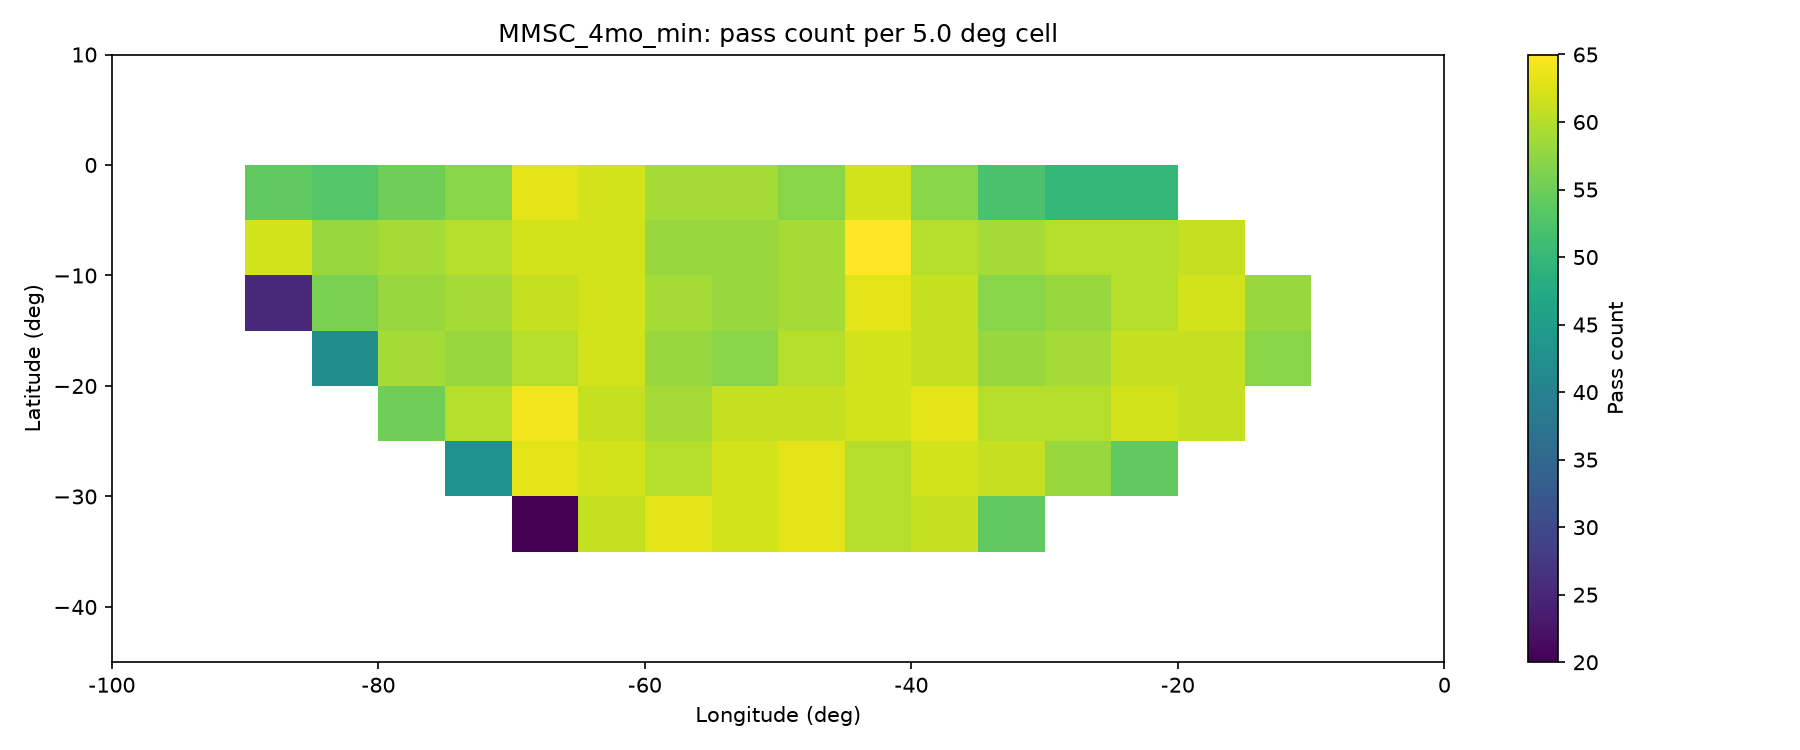
\includegraphics[width=.78\linewidth]{media/mmsc_4mo.png}\caption{Four-month MMSC science-grid output from the supplied simulation archive; model-dependent.}\label{fig:new-mmsc}\end{figure}
\begin{figure}[htbp]\centering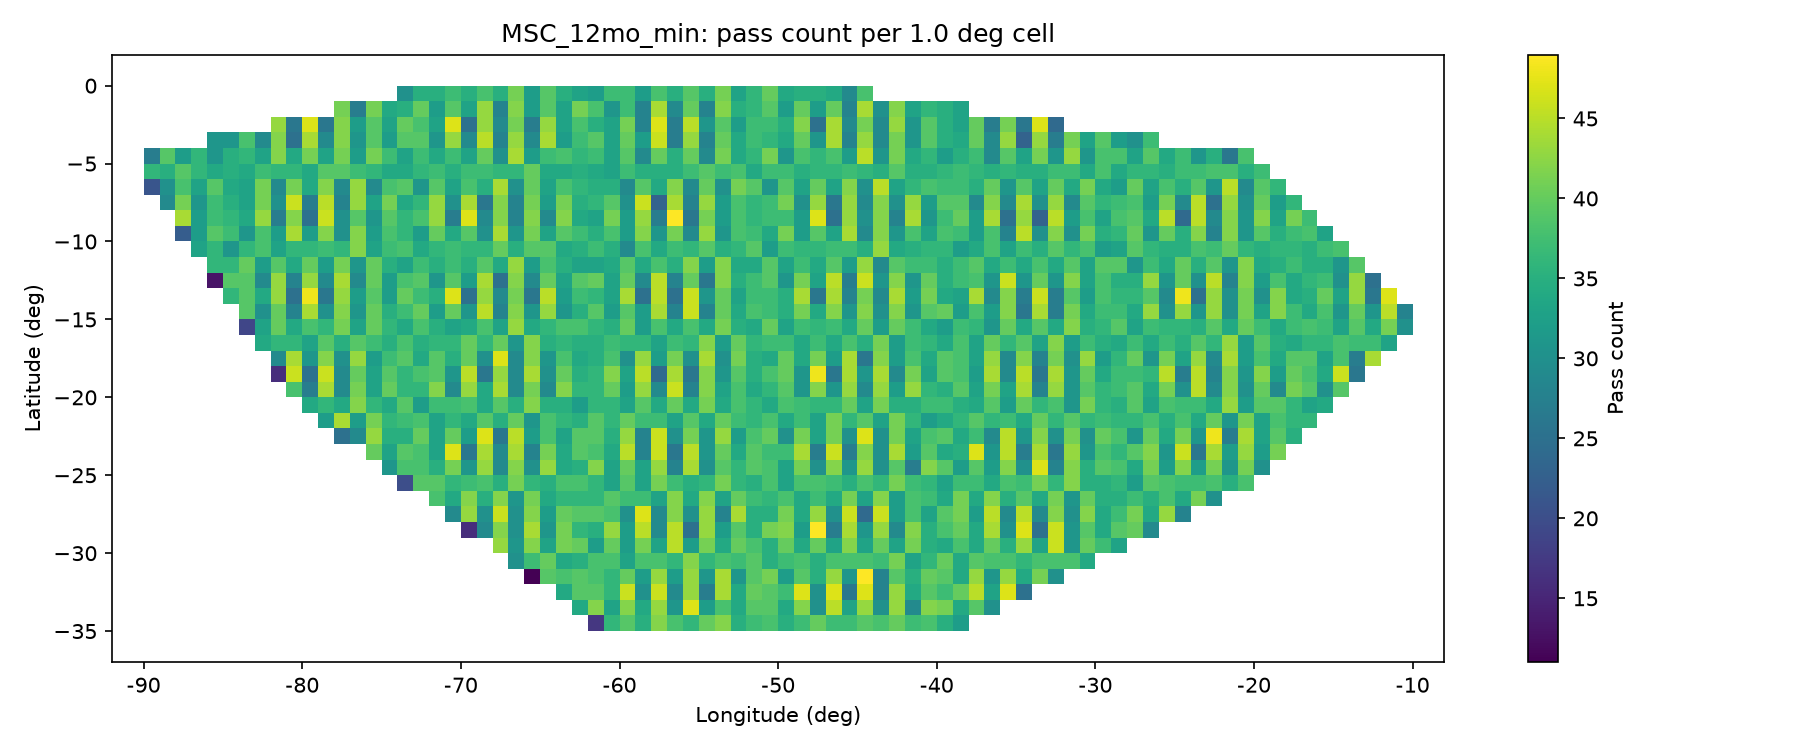
\includegraphics[width=.78\linewidth]{media/msc_12mo.png}\caption{Twelve-month MSC science-grid output from the supplied simulation archive; model-dependent.}\label{fig:new-msc}\end{figure}
\begin{figure}[htbp]\centering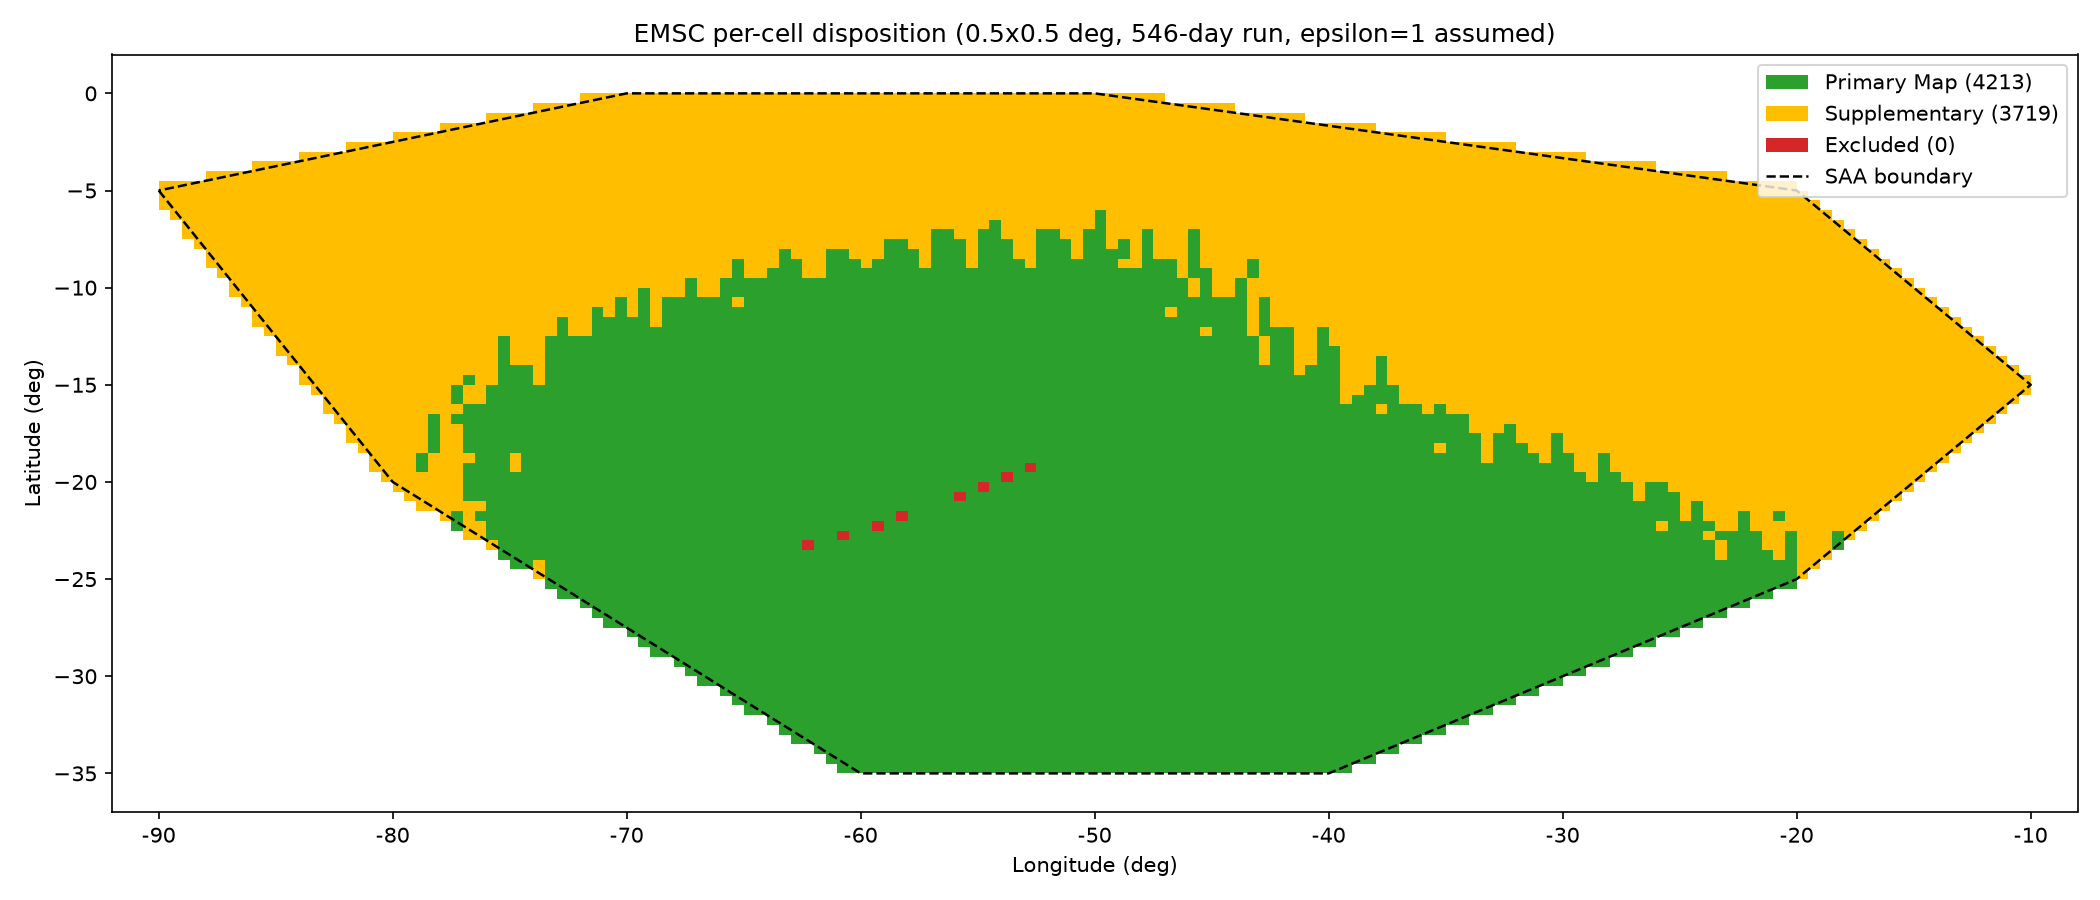
\includegraphics[width=.78\linewidth]{media/emsc.png}\caption{Extended science-grid classification from the supplied simulation archive; model-dependent.}\label{fig:new-emsc}\end{figure}

\subsection{Radiation and detector science model}
The supplied IRENE-related inputs, proton-spectrum output, stopping-range plots and pile-up calculations support preliminary detector analysis. They do not establish a fully calibrated telescope geometry, dead-time limit, response matrix, or actual AP9 output from the integrated Science simulator. The integrated simulator's AP9-named quantity is a configured baseline. Current scintillator dimensions are fixed in Appendix~\ref{app:payload-detail}; accepted event rates and detector response remain unqualified. The supplied 2026 AP9/AE9 grid is reproduced independently and accepted for preliminary 2029 planning with its original epoch retained.
The separate November geometric-factor bundle supports the conditional counting requirements in Appendix~\ref{app:required-g}. Its AP9-labelled 65-threshold spectrum has no generating manifest; the verified date of the earlier AP9/AE9 archive must not be transferred to it. The supplied rate heatmap is an ideal integral-above-5~MeV rate proxy, not a detector-efficiency or required-$G$ map.
\begin{figure}[htbp]\centering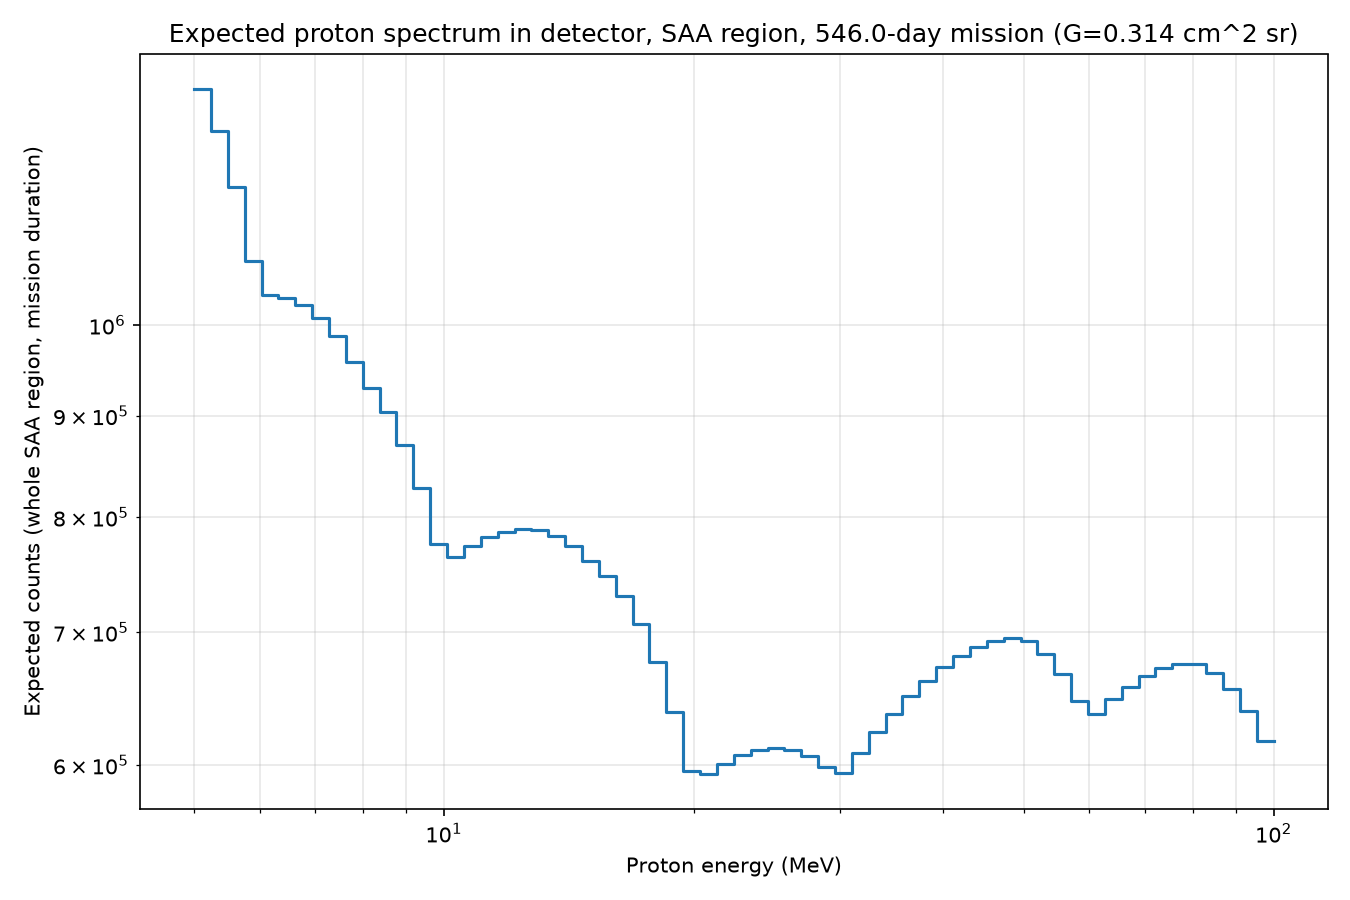
\includegraphics[width=.75\linewidth]{media/spectrum.png}\caption{Historical modeled SAA proton spectrum. Its title assumes 546 days and $G=0.314$~cm$^2$~sr; these labels do not verify runtime duration or connect it to the new unit-$G$ table. This is not a validated detector measurement.}\label{fig:new-spectrum}\end{figure}

\subsection{Ground-station and DITL source files}
The earlier historical one-day run (distinct from the newly supplied one-hour exports) includes six recorded SAA passages, two Goa ground-station contacts, one initial detumble event lasting 2460~s, and eighteen slew events. Contact durations are approximately 368 and 414~s. This is a historical run with an epoch of March 2000; its performance is not automatically representative of a late-2028 or early-2029 mission epoch. The complete telemetry CSV and event tables are retained externally as raw evidence.

\subsection{Preliminary procurement and mass allocation}
The uploaded bill of materials identifies candidate ADCS, OBC, solar-array, EPS, structure, communications, navigation and antenna parts. The sum of currently specified component-mass entries is 1536.3~g. The payload and deployer-interface hardware do not have mass entries, and the deployable-panel quantity and overall packaging need review. Consequently the bill of materials cannot yet close the mission target of less than 3000~g. Procurement prices remain to be supplied.

\subsection{Manufacturer documentation and CAD inputs}
Manufacturer documents were supplied for the ISISPACE ICEPS2, TensorTech integrated ADCS, GomSpace NanoMind A3200 and NanoCom AX100, 2nd Space CORE/DROP/VERSE hardware and the proposed GNSS components. CAD inputs were supplied for several candidate components. Final mechanical envelopes, actuator configurations, harness allowances and interface drawings must be checked against the actual proposed configuration before the component baselines become final.

\subsection{Remaining verification conditions}\label{sec:new-evidence-open}
\begin{longtable}{p{0.10\linewidth}p{0.47\linewidth}p{0.34\linewidth}}\caption{Open evidence required for MCR closure}\label{tab:new-open}\\\toprule ID & Open item & Needed evidence \\
\midrule\endfirsthead\toprule ID & Open item & Needed evidence \\
\midrule\endhead
O-01 & Reconcile historical SAA counter & New two-run orbit classifications are internally consistent; establish classifier geometry and event definitions \\
O-02 & 2029 campaign identity and RAAN robustness & Runtime manifests and environment timestamps for the team-accepted reference \\
O-03 & Long-term drag and disposal & Verify new 8--10-year cutoff runs, one truncated case, and post-cutoff reentry \\
O-04 & Solar area, efficiency, degradation and EOL margin & Approved solar/EPS report from final configuration \\
O-05 & FPDU response and electronics & Current CAD, optical isolation, transport, timing and mixed-species trigger validation \\
O-06 & Science-tier coverage requirements & Consistent geographic denominator, per-channel uncertainties and pass requirements \\
O-07 & Ground station RF and data-rate closure & Final payload packets, coding, link and antenna design \\
O-08 & Thermal and structural margins & Model outputs checked against component limits; tests planned \\
O-09 & Complete spacecraft mass and cost & Payload, wiring, deployment items, quantities and quotations \\
O-10 & Integrated long-term and scenario verification & Approved output files, code revision and run parameters \\
\bottomrule\end{longtable}

\subsection{Bill of materials, as supplied}\label{sec:bom-from-upload}
The following values are transcribed from the uploaded \texttt{BILL OF MATERIALS.xlsx}. Components are candidates, and none of the unresolved part numbers or interfaces is to be regarded as a final PDR selection. Values of ``TBD'' have not been imputed.
\begin{longtable}{p{0.23\linewidth}p{0.48\linewidth}p{0.08\linewidth}p{0.10\linewidth}}
\caption{Candidate component mass entries from supplied bill of materials}\label{tab:bom-upload}\\
\toprule Subsystem & Component or part & Qty. & Mass (g) \\\midrule\endfirsthead
\toprule Subsystem & Component or part & Qty. & Mass (g) \\\midrule\endhead
ADCS & ADCS-10m  & 1 & 495 \\
OBC & NanoMind A3200 & 1 & 24 \\
Power Generation & Core 1Z & 1 & 114 \\
Power Generation & DROP & 1 & 118 \\
EPS & ICEPS 2S1P+iEPS Battery Type A & 1 & 189 \\
Structure & Verse-03 & 1 & 310 \\
Communications & NanoCom AX100 & 1 & 24.5 \\
Communications & UHF dipole antenna & 1 & 90 \\
Communications & ANT430 & 1 & 30 \\
Deployment & TBD & 1 & TBD \\
Payload & Custom & 1 & TBD \\
Navigation & ZED-F9P-15B & 1 & 1.8 \\
Navigation & AHP54510.07.0100C & 1 & 140 \\
\bottomrule\end{longtable}
The workbook reports a total of 1536.3~g of currently entered masses, before adding the unallocated payload and deployment-interface mass. The current solar-panel quantity entries require confirmation against the intended one fixed and two deployable panel geometry. Costs in the workbook are not quoted amounts.

\subsection{Datasheet alignment checks}\label{sec:databook-check}
The supplied ICEPS2 datasheet describes a 2S1P battery pack with nominal energy 28.8~Wh. The 25~Wh value remains the mission simulation planning capacity. The supplied TensorTech ADCS-10m datasheet explicitly describes a control-moment gyroscope configuration. Since ANTARA intends to use a reaction-wheel and magnetorquer integrated system, that datasheet cannot be treated as proof of the selected ADCS hardware configuration. A matching vendor model and specification must be supplied. The GNSS, radio, antenna, deployment-panel and structure datasheets are candidate mechanical/electrical references, pending interface selection.

\subsection{Approved 2029 Planning Baseline}
\label{app:latest-baseline}
The mission reference is 1 January 2029: 3U, maximum 3.0~kg, approximately 600~km SSO, $97.6^\circ$ inclination, eccentricity approximately 0.001, launch-dependent RAAN, 25~Wh battery planning capacity and reaction wheels with magnetorquers. The team accepts the supplied RAAN data for 2029 planning; the inspected local MCR runtime still starts in 2026, so its generating epoch remains unverified. This does not prevent use as a clearly identified preliminary reference. The supplied radiation map retains its verified 2026 source epoch.

The approved FPDU has five longitudinal main blocks and one front scintillator, eleven SiPMs, no silicon entrance and optional rear detection. Optical isolation, material, calibrated response and processor selection remain open. Appendix~\ref{app:payload-detail} controls current construction and timing. Approximately five years is the operational objective; modeled decay to 300~km and subsequent reentry are separate quantities. The 8--10-year cutoff study retains its configuration and censoring limitations (Appendix~\ref{app:updated-raan}).
